\documentclass{beamer}

% https://tex.stackexchange.com/a/435104
\setbeamertemplate{frametitle continuation}{}

\usetheme{AnnArbor}

\def\OPTIONConf{1}
\usepackage{joshuadunfield}
\usepackage{llproof}
% !TEX root = hazelnut-popl17.tex

% Violet hotdogs; highlight color helps distinguish them
\newcommand{\llparenthesiscolor}{\textcolor{violet}{\llparenthesis}}
\newcommand{\rrparenthesiscolor}{\textcolor{violet}{\rrparenthesis}}

% HTyp and HExp
\newcommand{\hcomplete}[1]{#1~\mathsf{complete}}

% HTyp
\newcommand{\htau}{\dot{\tau}}
\newcommand{\tarr}[2]{\inparens{#1 \rightarrow #2}}
\newcommand{\tarrnp}[2]{#1 \rightarrow #2}
\newcommand{\tnum}{\mathtt{num}}
\newcommand{\tehole}{\llparenthesiscolor\rrparenthesiscolor}
\newcommand{\tsum}[2]{\inparens{{#1} + {#2}}}

\newcommand{\tcompat}[2]{#1 \sim #2}
\newcommand{\tincompat}[2]{#1 \nsim #2}

% HExp
\newcommand{\hexp}{\dot{e}}
\newcommand{\hlam}[2]{\inparens{\lambda #1.#2}}
\newcommand{\hap}[2]{#1(#2)}
\newcommand{\hapP}[2]{(#1)~(#2)} % Extra paren around function term
\newcommand{\hnum}[1]{\underline{#1}}
\newcommand{\hadd}[2]{\inparens{#1 + #2}}
\newcommand{\hehole}{\llparenthesiscolor\rrparenthesiscolor}
\newcommand{\hhole}[1]{\llparenthesiscolor#1\rrparenthesiscolor}
\newcommand{\hindet}[1]{\lceil#1\rceil}
\newcommand{\hinj}[2]{\mathtt{inj}_{#1}({#2})}
\newcommand{\hcase}[5]{\mathtt{case}({#1},{#2}.{#3},{#4}.{#5})}

\newcommand{\hGamma}{\dot{\Gamma}}
\newcommand{\domof}[1]{\text{dom}(#1)}
\newcommand{\hsyn}[3]{#1 \vdash #2 \Rightarrow #3}
\newcommand{\hana}[3]{#1 \vdash #2 \Leftarrow #3}

% ZTyp and ZExp
\newcommand{\zlsel}[1]{{\bowtie}{#1}}
\newcommand{\zrsel}[1]{{#1}{\bowtie}}
\newcommand{\zwsel}[1]{
  \setlength{\fboxsep}{0pt}
  \colorbox{green!10!white!100}{
    \ensuremath{{{\textcolor{Green}{{\hspace{-2px}\triangleright}}}}{#1}{\textcolor{Green}{\triangleleft{\vphantom{\tehole}}}}}}
}

\newcommand{\removeSel}[1]{#1^{\diamond}}

% ZTyp
\newcommand{\ztau}{\hat{\tau}}

% ZExp
\newcommand{\zexp}{\hat{e}}

% Direction
\newcommand{\dParent}{\mathtt{parent}}
\newcommand{\dChildn}[1]{\mathtt{child}~\mathtt{{#1}}}
\newcommand{\dChildnm}[1]{\mathtt{child}~{#1}}

% Action
\newcommand{\aMove}[1]{\mathtt{move}~#1}
	\newcommand{\zrightmost}[1]{\mathsf{rightmost}(#1)}
	\newcommand{\zleftmost}[1]{\mathsf{leftmost}(#1)}
\newcommand{\aSelect}[1]{\mathtt{sel}~#1}
\newcommand{\aDel}{\mathtt{del}}
\newcommand{\aReplace}[1]{\mathtt{replace}~#1}
\newcommand{\aConstruct}[1]{\mathtt{construct}~#1}
\newcommand{\aConstructx}[1]{#1}
\newcommand{\aFinish}{\mathtt{finish}}

\newcommand{\performAna}[5]{#1 \vdash #2 \xlongrightarrow{#4} #5 \Leftarrow #3}
\newcommand{\performAnaI}[5]{#1 \vdash #2 \xlongrightarrow{#4}\hspace{-3px}{}^{*}~ #5 \Leftarrow #3}
\newcommand{\performSyn}[6]{#1 \vdash #2 \Rightarrow #3 \xlongrightarrow{#4} #5 \Rightarrow #6}
\newcommand{\performSynI}[6]{#1 \vdash #2 \Rightarrow #3 \xlongrightarrow{#4}\hspace{-3px}{}^{*}~ #5 \Rightarrow #6}
\newcommand{\performTyp}[3]{#1 \xlongrightarrow{#2} #3}
\newcommand{\performTypI}[3]{#1 \xlongrightarrow{#2}\hspace{-3px}{}^{*}~#3}

\newcommand{\performMove}[3]{#1 \xlongrightarrow{#2} #3}
\newcommand{\performDel}[2]{#1 \xlongrightarrow{\aDel} #2}

% Form
\newcommand{\farr}{\mathtt{arrow}}
\newcommand{\fnum}{\mathtt{num}}
\newcommand{\fsum}{\mathtt{sum}}

\newcommand{\fasc}{\mathtt{asc}}
\newcommand{\fvar}[1]{\mathtt{var}~#1}
\newcommand{\flam}[1]{\mathtt{lam}~#1}
\newcommand{\fap}{\mathtt{ap}}
% \newcommand{\farg}{\mathtt{arg}}
\newcommand{\fnumlit}[1]{\mathtt{lit}~#1}
\newcommand{\fplus}{\mathtt{plus}}
\newcommand{\fhole}{\mathtt{hole}}
\newcommand{\fnehole}{\mathtt{nehole}}

\newcommand{\finj}[1]{\mathtt{inj}~#1}
\newcommand{\fcase}[2]{\mathtt{case}~#1~#2}

% Talk about formal rules in example
\newcommand{\refrule}[1]{\textrm{Rule~(#1)}}

\newcommand{\herase}[1]{\left|#1\right|_\textsf{erase}}

\newcommand{\arrmatch}[2]{#1 \blacktriangleright_{\rightarrow} #2}


\newcommand{\TABperformAna}[5]{#1 \vdash & #2                & \xlongrightarrow{#4} & #5 & \Leftarrow #3}
\newcommand{\TABperformSyn}[6]{#1 \vdash & #2 \Rightarrow #3 & \xlongrightarrow{#4} & #5 \Rightarrow #6}
\newcommand{\TABperformTyp}[3]{& #1 & \xlongrightarrow{#2} & #3}

\newcommand{\TABperformMove}[3]{#1 & \xlongrightarrow{#2} & #3}
\newcommand{\TABperformDel}[2]{#1 \xlongrightarrow{\aDel} #2}

\newcommand{\sumhasmatched}[2]{#1 \mathrel{\textcolor{black}{\blacktriangleright_{+}}} #2}

\newcommand{\subminsyn}[1]{\mathsf{submin}_{\Rightarrow}(#1)}
\newcommand{\subminana}[1]{\mathsf{submin}_{\Leftarrow}(#1)}


\newcommand{\inparens}[1]{{\color{gray}(}#1{\color{gray})}}

%% rule names for appendix
\newcommand{\rname}[1]{\textsc{#1}}
\newcommand{\gap}{\vspace{7pt}}

% for header page
\newcommand{\vs}{\vspace{20pt}}

% for header page
\newcommand{\pt}[1]{\MakeUppercase{
    \centering{}
    \large{}
    #1 \\
    \vs{}
  }}

% allow custom lexer for pygmentize
% https://github.com/gpoore/minted/issues/176#issuecomment-695344998
\usepackage{minted}
\usepackage{regexpatch}

\makeatletter
\newcommand{\minted@def@optcl@novalue}[2]{%
  \define@key{minted@opt@g}{#1}[]{%
    \minted@addto@optlistcl{\minted@optlistcl@g}{#2}%
    \@namedef{minted@opt@g:#1}{#2}}%
  \define@key{minted@opt@g@i}{#1}[]{%
    \minted@addto@optlistcl{\minted@optlistcl@g@i}{#2}%
    \@namedef{minted@opt@g@i:#1}{#2}}%
  \define@key{minted@opt@lang}{#1}[]{%
    \minted@addto@optlistcl@lang{minted@optlistcl@lang\minted@lang}{#2}%
    \@namedef{minted@opt@lang\minted@lang:#1}{#2}}%
  \define@key{minted@opt@lang@i}{#1}[]{%
    \minted@addto@optlistcl@lang{%
      minted@optlistcl@lang\minted@lang @i}{#2}%
    \@namedef{minted@opt@lang\minted@lang @i:#1}{#2}}%
  \define@key{minted@opt@cmd}{#1}[]{%
    \minted@addto@optlistcl{\minted@optlistcl@cmd}{#2}%
    \@namedef{minted@opt@cmd:#1}{#2}}%
}

% new minted option "custom" for adding command line option "-x"
\minted@def@optcl@novalue{custom}{-x}

% new minted option "formatter=<formatter>" for specifying pygments formatter
\minted@def@opt{formatter}

% apply "-f <formatter>"
\newcommand\minted@formatter{%
  \minted@get@opt{formatter}{latex}\space
}

% Note: may require fix to regexpatch:
% https://tex.stackexchange.com/questions/578518/regexpatchcmd-failing-with-latex2e-2020-10-01-patch-level-4-use-cs-replacemen#comment1469403_578518
\xpatchcmd*\minted@checkstyle
  {-f latex }
  {-f \minted@formatter}
  {}{\fail}
\xpatchcmd*\minted@pygmentize
  {-f latex }
  {-f \minted@formatter}
  {}{\fail}

  \makeatother
  % end custom lexer for pygmatize

% Need VerbatimEnvironment:
% https://tex.stackexchange.com/a/400115
\newenvironment{hminted}
{\VerbatimEnvironment
\begin{minted}[escapeinside=//,frame=single,custom]{../latex-includes/hazel_lexer.py:HazelLexer}}
{\end{minted}}

% hazel inline; don't really know what's going on here
% https://tex.stackexchange.com/a/181393
\newcommand{\hmintinlinet}{
  \mintinline[escapeinside=//,frame=single,custom]{../latex-includes/hazel_lexer.py:HazelLexer}
}
\newcommand{\hmintinline}[1]{\expandafter\hmintinlinet\expandafter{#1}}

% \newcommand{\ab}{expanded stuff}
% \newcommand{\pythoninline}{\mintinline[]{python}}

% hazel inputminted
\newcommand{\inputhminted}[1]{\inputminted[escapeinside=//,frame=single,custom]{../latex-includes/hazel_lexer.py:HazelLexer}{lstings/#1.hz}}

% ocaml inputminted
\newcommand{\inputominted}[1]{\inputminted[escapeinside=//,frame=single]{ocaml}{lstings/#1.ml}}


% extra math operators
% especially for math operators that are introduced in this paper, want to
% declare them here so they are easily changeable
\DeclareMathOperator{\fix}{fix}       % fixpoint
\newcommand{\env}{\sigma}             % environment
\newcommand{\pp}{\Uparrow}            % post-process
\newcommand{\pplc}{\pp_{[]}}          % post-process lambda conversion (substitution) operator
\newcommand{\pplco}{\pp_{[],1}}       % post-process lc part 1
\newcommand{\pplct}{\pp_{[],2}}       % post-process lc part 2
\newcommand{\ppn}{\pp_{i}}            % post-process hole closure numbering
\newcommand{\ppnd}{\pp_{i,d}}         % post-process hole closure numbering (results only)
\newcommand{\ppns}{\pp_{i,\env}}      % post-process hole closure numbering (sigmas only)
\newcommand{\pplcl}{PPI$_{[]}$}       % post-process lambda within evaluation boundary conversion label
\newcommand{\pplclo}{PPO$_{[]}$}      % post-process lambda outside evaluation boundary conversion label
\newcommand{\ppndl}{PP$_{i,d}$}       % post-process hole closure numbering label
\newcommand{\ppnsl}{PP$_{i,\env}$}     % post-process hole closure numbering label
\newcommand{\pth}{p}                  % path
\newcommand{\hci}{H}                  % hole instance/closure info
\DeclareMathOperator{\hid}{hid}       % hole instance id generator

% for use in Hazel listings
\newcommand{\rar}{$\rightarrow$}
\newcommand{\Rar}{$\Rightarrow$}
\newcommand{\lbd}{$\lambda$}
\newcommand{\heh}[1]{$\hehole^{#1}$}

% for missing references
\newcommand{\todo}[1]{\textbf{[TODO: #1]}}
\newcommand{\todoref}[1]{\textbf{[TODO: need reference(s): #1]}}

%%% Local Variables:
%%% mode: latex
%%% TeX-master: "../thesis/main"
%%% End:


\newtheorem{mtheorem}{Metatheorem}[section]

\usepackage{adjustbox}

\title[Hazel evaluation improvements]{Practical performance enhancements to the evaluation model of the Hazel programming environment}

\author[Lam]
{
  Jonathan~Lam\inst{1} \and Prof. Fred Fontaine, Advisor\inst{1} \\
  \and Prof. Robert Marano, Co-advisor\inst{1} \and Prof. Cyrus Omar\inst{2}
}

\institute[Cooper Union]
{
  \inst{1}%
  Electrical Engineering\\
  The Cooper Union for the Advancement of Science and Art
  \and
  \inst{2}%
  Electrical Engineering and Computer Science\\
  Future of Programming Lab (FPLab), University of Michigan
}

\date[Spring 2022]{2022/04/29}

% https://www.overleaf.com/learn/latex/Beamer
\AtBeginSection[]
{
  \begin{frame}
    \frametitle{Table of Contents}
    \tableofcontents[currentsection]
  \end{frame}
}

\begin{document}

\frame{\titlepage}

\begin{frame}[allowframebreaks]
  \frametitle{Overview}

  Project context
  \begin{description}
  \item[Hazel live programming environment] An experimental editor with typed holes aimed at solving the ``gap problem,'' developed at UM
  \item[Functional programming] Context for PL theory
  \item[Implementation-based] Mostly practically-driven
  \end{description}

  \vspace{4em}
  Project goal
  \begin{description}
  \item[Improve aspects of Hazel evaluation] Mostly performance-related
  \end{description}

  \vspace{12em} Project scope
  \begin{description}
  \item[Evaluation with environments] Lazy variable lookup for performance
  \item[Hole instances to hole closures] Redefining hole instances for performance
  \item[Implementing fill-and-resume (FAR)] Efficiently resume evaluation
  \end{description}

  \vspace{4em}Project evaluation
  \begin{description}
  \item[Empirical evaluation] Measure performance gain of motivating cases
  \item[Informal metatheory] State metatheorems and provide proof sketches
  \end{description}
\end{frame}

\section{Primer on PL theory}

\begin{frame}
  \frametitle{A programming language is a specification}

  \begin{description}
  \item[Syntax] is the grammar of a valid program
  \item[Semantics] describes the behavior of a syntactically valid program
  \end{description}

  \begin{figure}
    \centering
    \begin{align*}
  \tau &::= \tau\to\tau
         \mid b
         \mid \tehole \\
  e &::= c
      \mid x
      \mid\lambda x:\tau.e
      \mid e\ e
      \mid e:\tau
      \mid \hehole
      \mid \hhole{e}
\end{align*}

    \caption{Hazelnut grammar}
    \label{fig:hazelnut-grammar}
  \end{figure}

\end{frame}

\begin{frame}
  \frametitle{Static and dynamic semantics}

  \begin{description}
  \item[Statics] Edit actions, type-checking, elaboration (``compile-time'')
  \item[Dynamics] Evaluation (``run-time'')
  \end{description}

  \begin{figure}
    \centering
    \begin{mathpar}
      \Infer{EAp}{\
        e_1\Downarrow \lambda x.e_1' \\
        e_2\Downarrow e_2' \\
        [e_2'/x]e_1'\Downarrow e
      }{e_1\ e_2\Downarrow e}
    \end{mathpar}
    \caption{Evaluation rule for function application using a big-step semantics}
    \label{fig:inference-rules}
  \end{figure}
\end{frame}

\begin{frame}
  \frametitle{A brief primer on the $\lambda$-calculus}

  \begin{description}
  \item[Untyped $\lambda$-calculus] Simple universal model of computation by Church
    % not relevant
    % \item[Simply-typed $\lambda$-calculus] Extension of the ULC with static type-checking
    % \item[Gradually-typed $\lambda$-calculus] Optionally-typed, with ``pay-as-you-go'' benefits of static typing
  \end{description}

  \begin{figure}
    \centering
    \begin{subfigure}[b]{.2\textwidth}
        \begin{align*}
          e &::= x\\
            &\mid \lambda x.e\\
            &\mid e\ e
        \end{align*}
      \caption{Grammar}
    \end{subfigure}\qquad
    \begin{subfigure}[b]{.7\textwidth}
      \begin{mathpar}
  \Infer{\ulc{}-ELam}{}{\lambda x.e\Downarrow\lambda x.e}
  \and
  \Infer{\ulc{}-EAp}{
    e_1\Downarrow\lambda x.e_1' \\
    [e_2/x]e_1'\Downarrow e
  }{e_1\ e_2\Downarrow e}
\end{mathpar}

      \caption{Dynamic semantics}
    \end{subfigure}
    \caption{The untyped $\lambda$-calculus}
    \label{fig:ulc}
  \end{figure}
\end{frame}

\section{The Hazel live programming environment}

\begin{frame}
  \frametitle{The Hazel programming language and environment}

  \begin{description}
  \item[Live programming] Rapid static and dynamic feedback (``gap problem'')
  \item[Structured editor] Elimination of syntax errors
  \item[Gradually typed] Hole type and cast-calculus based on Siek et al. \cite{Siek06gradualtyping,siek2015refined}
  \item[Purely functional] Avoids side-effects and promotes commutativity
  \end{description}

  \begin{figure}
    \centering
    \begin{subfigure}[b]{0.5\textwidth}
      \centering
      
\includegraphics[height=5em]{thesis/img/hazelgrove.png}
      \caption{The Hazelgrove organization}
    \end{subfigure}%
    \begin{subfigure}[b]{0.5\textwidth}
      \centering
      
\includegraphics[height=5em]{thesis/img/reasonml.png}
      \caption{Implemented in ReasonML and JSOO}
    \end{subfigure}
    \caption{Hazel implementation}
  \end{figure}
\end{frame}

\begin{frame}
  \frametitle{The Hazel programming interface}

  \begin{figure}
    \centering
    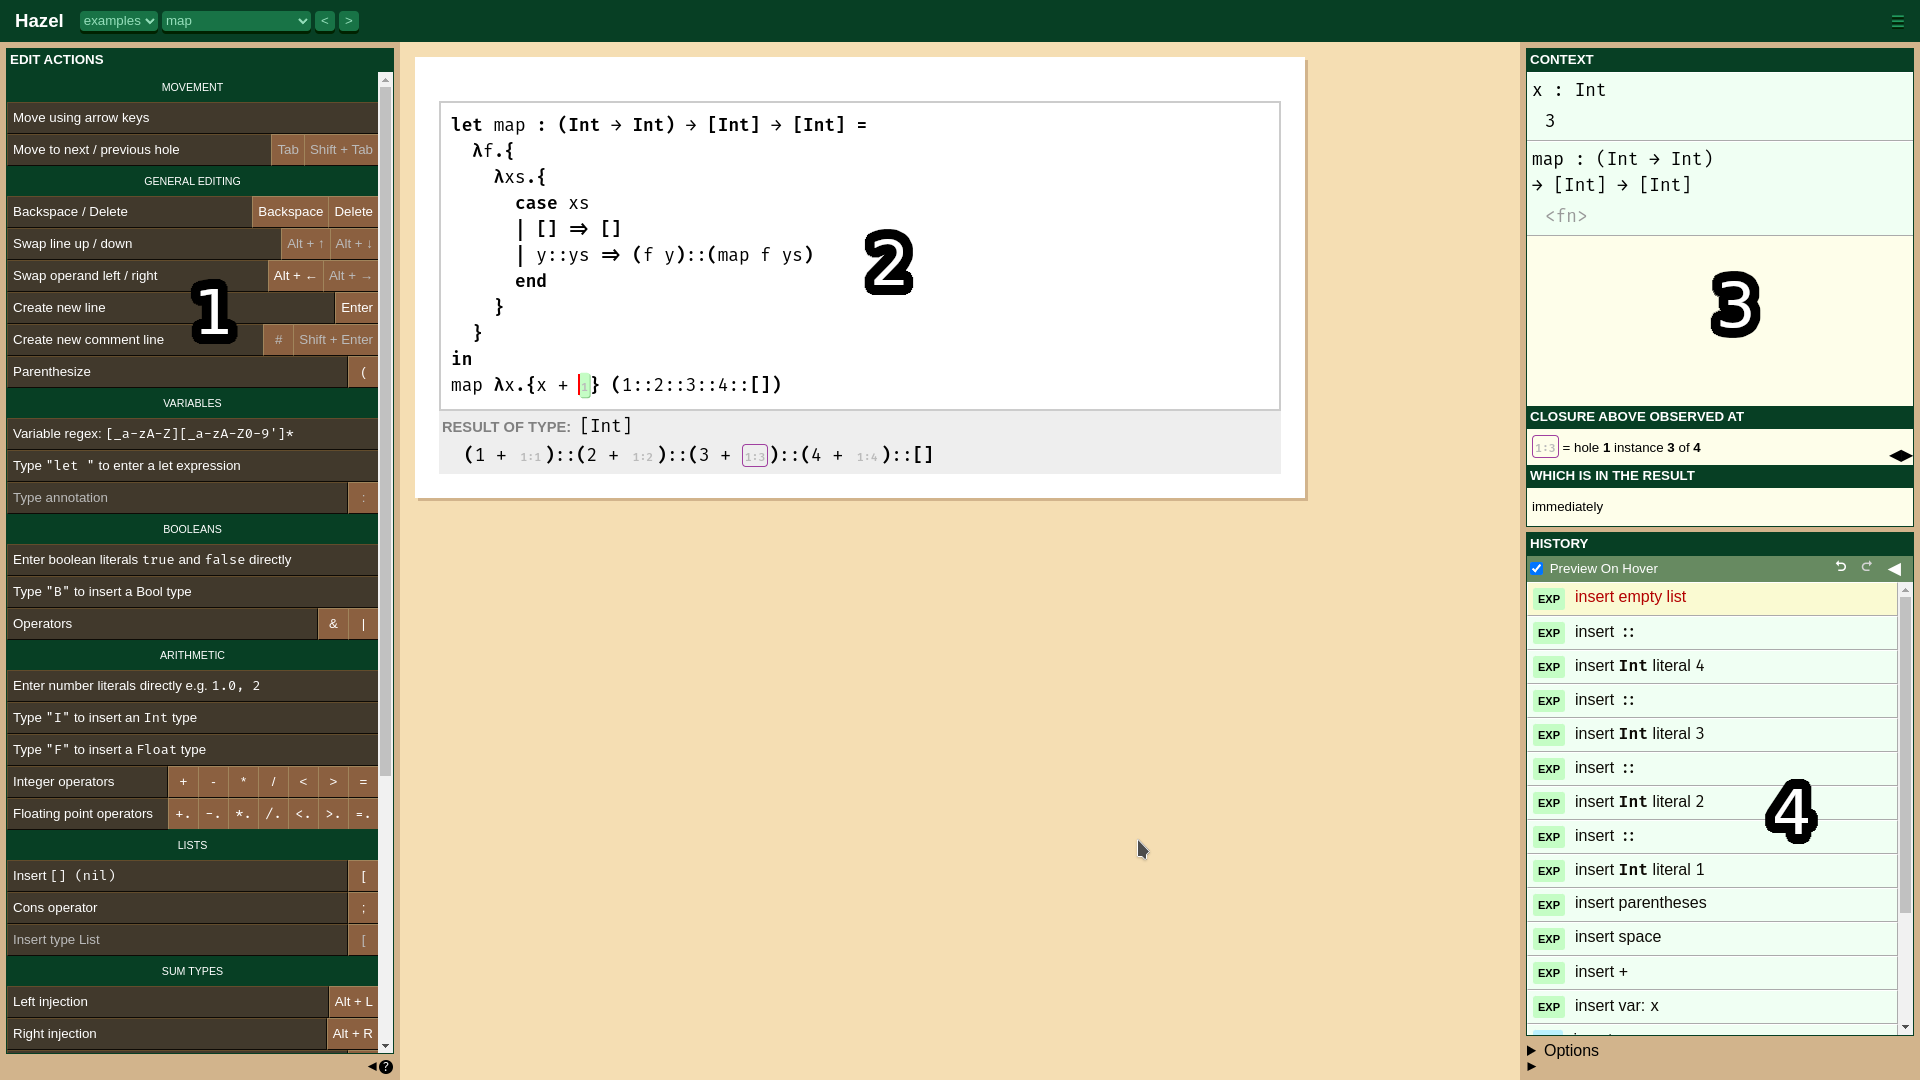
\includegraphics[width=.9\linewidth]{thesis/img/hazel_ui_annot.png}
    \caption{The Hazel interface}
    \label{fig:hazel-ui}
  \end{figure}

\end{frame}

\begin{frame}
  \frametitle{Hazelnut: A bidirectionally-typed static semantics}

  \begin{description}
  \item[(Typed) expression holes] Internalize ``red squiggly underlines''
  \item[Action semantics] Structural editing behavior, ensures always well-typed
  \end{description}

  \begin{figure}
    \centering
    \begin{subfigure}[b]{0.45\textwidth}
      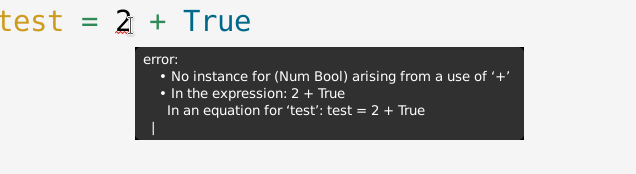
\includegraphics[width=\textwidth]{thesis/img/haskell_squiggle}
      \caption{Haskell static type error}
    \end{subfigure}
    \qquad
    \begin{subfigure}[b]{0.45\textwidth}
      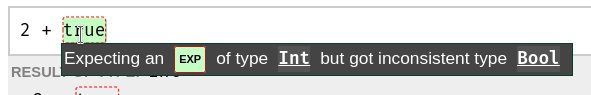
\includegraphics[width=\textwidth]{thesis/img/hazel_squiggle}
      \caption{Hazel non-empty hole}
    \end{subfigure}
    \caption{``Red squiggly underline''}
    % 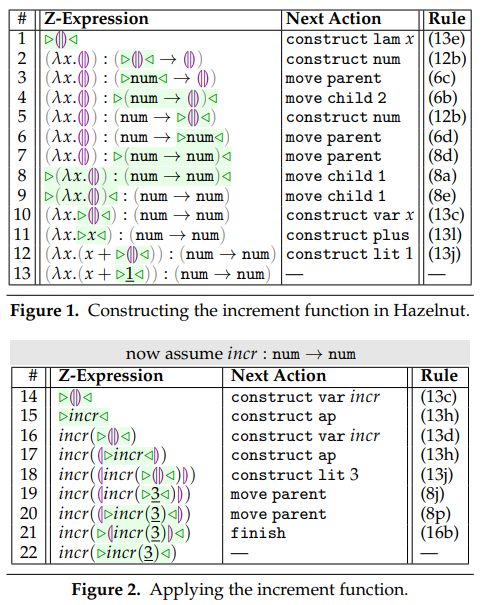
\includegraphics[width=10em]{thesis/img/hazelnut_actions}
    % \caption{Sample Hazelnut action sequence \cite{conf/popl/Hazelnut17}}
    \label{fig:hazelnut-action-sequence}
  \end{figure}
\end{frame}

\begin{frame}
  \frametitle{Hazelnut Live: A bidirectionally-typed dynamic semantics}

  \begin{description}
  \item[Internal language] Cast calculus from Siek et al. \cite{Siek06gradualtyping,siek2015refined} for dynamic typing
  \item[Hole evaluation] Evaluation continues \textit{around} holes, captures environment
  \end{description}
  
  \begin{figure}
    \centering
    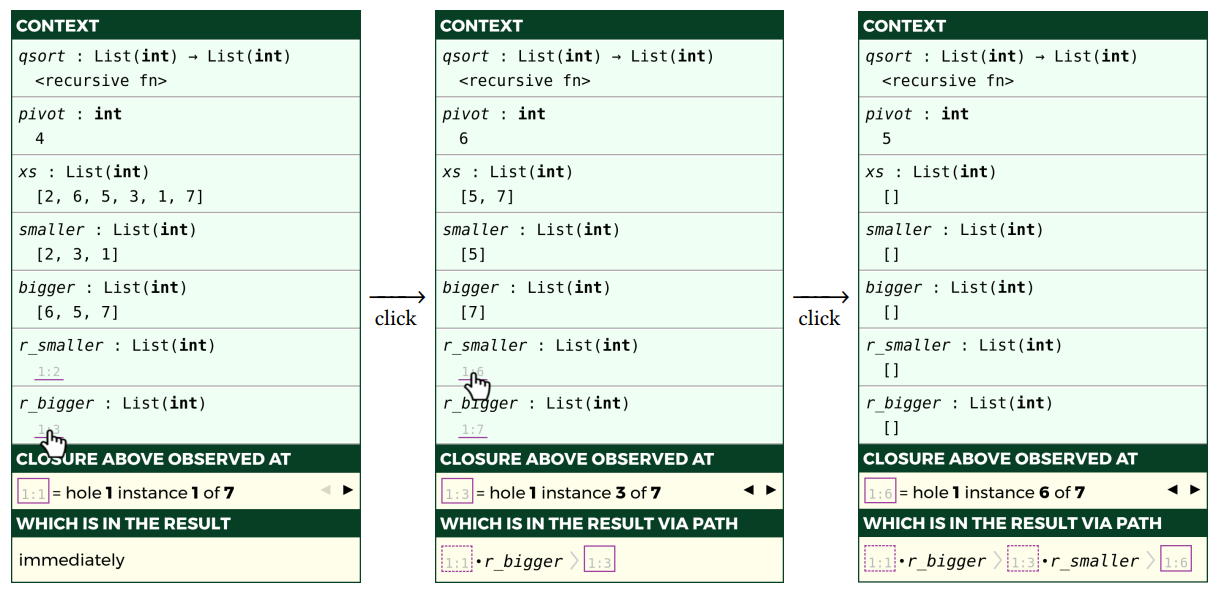
\includegraphics[height=10em]{thesis/img/hazelnut_live_context_inspector}
    \caption{Illustration of Hazelnut Live context inspector \cite{conf/popl/HazelnutLive19}}
    \label{fig:hazelnut-live-context-inspector}
  \end{figure}
\end{frame}

\section{Evaluation using the environment model}

\begin{frame}
  \frametitle{Evaluation using environments vs. substitution}

  \begin{figure}
    \centering
    \begin{subfigure}[b]{0.45\textwidth}
      \begin{align*}
        & \texttt{let }x=3\texttt{ in}\\
        & \texttt{if True then }0\texttt{ else }x
      \end{align*}
      \caption{Expression with variable binding}
    \end{subfigure} \\
    \begin{subfigure}[b]{0.35\textwidth}
      \begin{equation*}
        \texttt{if True then }0\texttt{ else }3
      \end{equation*}
      \caption{Substitution (eager)}
    \end{subfigure}
    \qquad
    \begin{subfigure}[b]{0.55\textwidth}
      \begin{equation*}
        \{x\leftarrow 3\}\vdash(\texttt{if True then }0\texttt{ else }x)
      \end{equation*}
      \caption{Environments (lazy)}
    \end{subfigure}
    \caption{Comparison of variable binding methods}
  \end{figure}
\end{frame}

\begin{frame}
  \frametitle{Updated evaluation rules}

  % \todo{include slide of evaluation rules with substitution}

  \begin{figure}
    \footnotesize
    \centering
    \judgbox{\env\vdash d\Downarrow d'}{$d$ evaluates to $d'$ given environment $\env$}

\begin{mathpar}
  \Infer{ELam}{}{\env\vdash(\lambda x:\tau.d)\Downarrow [\env](\lambda x:\tau.d')} \\
  \and
  \Infer{EVar}{}{\env,x\leftarrow d\vdash x\Downarrow d}
  \and
  \Infer{EAp}{
    \env\vdash d_1\Downarrow[\env']\lambda x:\tau.d_1' \\
    \env\vdash d_2\Downarrow d_2' \\
    \env',x\leftarrow d_2'\vdash d_1'\Downarrow d
  }{\env\vdash d_1\ d_2\Downarrow d}
  \and
  \Infer{EvalB-EHole}{}{\env\vdash\hehole^u\Downarrow[\env]\hehole^u}
  \and
  \Infer{EvalB-NEHole}{
    \env\vdash d\Downarrow d'
  }{\env\vdash\hhole{d}^u\Downarrow[\env]\hhole{d'}^u}
\end{mathpar}

%%% Local Variables:
%%% mode: latex
%%% TeX-master: "main"
%%% End:
    \caption{Big-step semantics for evaluation with environments}
    \label{fig:eval-env-rules}
  \end{figure}
\end{frame}

% extra
% \begin{frame}
%   \frametitle{Handling recursion}

%   \begin{description}
%   \item[Fixpoint form] Useful for a pure implementation of recursive functions, from Plotkin's System PCF
%   \end{description}
  
%   \begin{figure}
%     \footnotesize
%     \centering
%     \begin{mathpar}
  \Infer{EFix}{
    \env\vdash d\Downarrow [\env']d'
  }{
    \env\vdash\fix f:\tau.d\Downarrow [\env,f\leftarrow\fix f:\tau.[\env']d']d'
  } \\
  \and
  \Infer{EVar}{d\ne\fix f:\tau.d'}{\env,x\leftarrow d\vdash x\Downarrow d}
  \and
  \Infer{EUnwind}{
    \env\vdash\fix f:\tau.d\Downarrow d'
  }{\env,x\leftarrow\fix f:\tau.d\vdash x\Downarrow d'}
\end{mathpar}

%%% Local Variables:
%%% mode: latex
%%% TeX-master: "main"
%%% End:

%     \caption{Big-step semantics for evaluation of fixpoints}
%     \label{fig:fixpoint-rules}
%   \end{figure}
% \end{frame}

\begin{frame}
  \frametitle{Matching the result from evaluation using substitution}

  \begin{figure}
    \centering
    \footnotesize
    \renewcommand{\judgboxfontsize}{\footnotesize}
    % this is for the presentation
\newcommand{\lsize}{\tiny}

\judgbox{d\pplc d'}{$d$ is substitutes to $d'$ inside the evaluation boundary}

\begin{mathpar}
  \Infer{\lsize\pplcl{}Const}{
  }{c\pplc c}
  \and
  \Infer{\lsize\pplcl{}Ap}{
    d_1\pplc d_1' \\
    d_2\pplc d_2'
  }{d_1\ d_2\pplc d_1'\ d_2'}
  \and
  \Infer{\lsize\pplcl{}Closure}{
    \env\pplc\env' \\
    \env'\vdash d\pplc d'
  }{[\env]d\pplc d'}
\end{mathpar}

\judgbox{\env\vdash d\pplc d'}{$d$ substitutes to $d'$ outside the evaluation boundary}

\begin{mathpar}
  \Infer{\lsize\pplclo{}Const}{
  }{c\pplc c}
  \and
  \Infer{\lsize\pplclo{}BoundVar}{}{\env,x\leftarrow d\vdash x\pplc d}
  \and
  \Infer{\lsize\pplclo{}UnboundVar}{
    x\not\in\env
  }{\env,\vdash x\pplc x}
  \and
  \Infer{\lsize\pplclo{}Lam}{
    \env\vdash d\pplc d'
  }{\env\vdash\lambda x.d\pplc\lambda x.d'}
  \and
  \Infer{\lsize\pplclo{}Ap}{
    \env\vdash d_1\pplc d_1' \\
    \env\vdash d_2\pplc d_2'
  }{\env\vdash d_1(d_2)\pplc d_1'(d_2')}
  \and
  \Infer{\lsize\pplclo{}EHole}{
  }{\env\vdash\hehole^u\pplc[\env]\hehole^u}
  \and
  \Infer{\lsize\pplclo{}NEHole}{
    \env\vdash d\pplc d'
  }{\env\vdash\hhole{d}^u\pplc[\env]\hhole{d'}^u}
\end{mathpar}

%%% Local Variables:
%%% mode: latex
%%% TeX-master: "main"
%%% End:
    \caption{Big-step semantics for substitution postprocessing}
    \label{fig:pplc-rules}
  \end{figure}
\end{frame}

\begin{frame}
  \frametitle{Generalized closures}

  Notation in \textcolor{blue}{blue} is non-standard
  
  \begin{table}
    \centering
    \begin{tabular}{l|l}
      \hline
      Interpretation & Sample expression \\
      \hline\hline
      Function closure & $[\env]\lambda x.d$ \\
      Hole closure & $\textcolor{blue}{[\env]}\hhole{d}^u$ \\
      Closure around unmatched \texttt{let} & $\textcolor{blue}{[\env]}(\texttt{let }x=d_1\texttt{ in }d_2)$ \\
      Closure around unmatched \texttt{case} & $\textcolor{blue}{[\env]}(\texttt{case }x\texttt{ of }\text{rules})$ \\
      Closure around filled hole & $\textcolor{blue}{\llbracket\env\rrbracket} d_{fill}$ \\
      \hline\hline
    \end{tabular}
    \caption{Examples of generalized closures}
    \label{tab:generaized-closures-examples}
  \end{table}

\end{frame}

\begin{frame}
  \frametitle{The evaluation boundary}
  % Closures denote either where evaluation stops, and/or where evaluation may be resumed
  % Evaluation boundary denotes where evaluation stops

  \begin{figure}
    \centering
    \begin{subfigure}[b]{0.45\textwidth}
      \tiny
      \inputhpminted{eval_boundary}
      \caption{Program}
    \end{subfigure}
    \qquad
    \begin{subfigure}[b]{0.45\textwidth}
      \tiny
      \begin{equation*}
        \Downarrow (2+[x\leftarrow 5]\hehole^1)+[a\leftarrow\dots]\hhole{[\varnothing](\lambda x.2+\hehole^1)}^2
      \end{equation*}
      \caption{Program result}
    \end{subfigure} \\
    
    \begin{subfigure}[b]{\textwidth}
      \centering
      \maxsizebox{\textwidth}{10em}{
        \begin{tikzpicture}
          \node[] (a) {$\cdot+\cdot$};
          \node[below left=1em and 4em of a] (b) {$\cdot+\cdot$};
          \node[below left=1em of b] (c) {$2$};
          \node[below right=1em of b] (d) {$[x\leftarrow 5]\cdot$};
          \node[below=1em of d] (e) {$\hehole^1$};
          \node[below right=1em and 4em of a] (f1) {$[a\leftarrow\dots]\cdot$};
          \node[below=1em of f1] (f) {$\hhole{\cdot}^2$};
          \node[below=1em of f] (g1) {$[\varnothing]\cdot$};
          \node[below=1em of g1] (g) {$\lambda x.\cdot$};
          \node[below=1em of g] (h) {$\cdot+\cdot$};
          \node[below left=1em of h] (i) {$2$};
          \node[below right=1em of h] (j) {$\hehole^1$};

          \draw[] (a) -- (b);
          \draw[] (b) -- (c);
          \draw[] (b) -- (d);
          \draw[] (d) -- (e);
          \draw[] (a) -- (f1);
          \draw[] (f1) -- (f);
          \draw[] (f) -- (g1);
          \draw[] (g1) -- (g);
          \draw[] (g) -- (h);
          \draw[] (h) -- (i);
          \draw[] (h) -- (j);

          % hardcoded coordinates -- eww
          \path[draw=blue,dotted,thick] (-5,-3.6) -- (5,-3.6);
          \path[draw=red,dotted,thick] (-1.5,-2.3) -- (-0.5,-2.3);
          \path[draw=red,dotted,thick] (2.5,-1.5) -- (3.5,-1.5);
        \end{tikzpicture}
      }
      \caption{Program result AST}
    \end{subfigure}
    \caption{Illustration of evaluation boundary}
  \end{figure}
\end{frame}

\section{Identifying hole instances by physical environment}

\begin{frame}
  \frametitle{Motivation for hole instances}

  \begin{figure}
    \inputhpminted{instance_illustration}
    \caption{Illustration of hole instances}
    \label{fig:instance-illustration}
  \end{figure}

  \begin{figure}
    \centering
    \begin{equation*}
      [a\leftarrow[\varnothing]\hehole^1,x\leftarrow 3]\hehole^2
      + [a\leftarrow[\varnothing]\hehole^1,x\leftarrow 4]\hehole^2
    \end{equation*}
    \caption{Result of \Cref{fig:instance-illustration}}
    \label{fig:hole-instance-result}
  \end{figure}
\end{frame}

\begin{frame}[allowframebreaks]
  \frametitle{Motivation for hole closures/instantiations}

  \begin{figure}
    \centering
    \inputhpminted{holes_consecutive}
    \caption{A Hazel program that generates $2^N$ total hole instances}
    \label{fig:hole-renumbering-problem}
  \end{figure}

  \begin{figure}
    \centering
    \begin{subfigure}[b]{0.3\textwidth}
      \centering
      \maxsizebox{\textwidth}{10em}{
        \begin{tikzpicture}
  \node[] (hole4) {$[\env^4]\hehole^4$};
  \node[below=of hole4] (hole3) {$[\env^3]\hehole^3$};
  \node[below=of hole3] (hole2) {$[\env^2]\hehole^2$};
  \node[below=of hole2] (hole1) {$[\varnothing]\hehole^1$};

  \draw[->] (hole4) -- node [midway,left] {$c$} (hole3);
  \draw[->] (hole4) to[bend left=60] node [midway,right] {$b$} (hole2);
  \draw[->] (hole4) to[bend left=80] node [midway,right] {$a$} (hole1);
  \draw[->] (hole3) -- node [midway,left] {$b$} (hole2);
  \draw[->] (hole3) to[bend right=60] node [midway,left] {$a$} (hole1);
  \draw[->] (hole2) -- node [midway,left] {$a$} (hole1);
\end{tikzpicture}

%%% Local Variables:
%%% mode: latex
%%% TeX-master: "main"
%%% End:

      }
      \caption{Structure of the result}
      \label{fig:hole-renumbering-solution-structure}
    \end{subfigure}
    \qquad
    \begin{subfigure}[b]{0.6\textwidth}
      \centering
      \maxsizebox{\textwidth}{10em}{
        \begin{tikzpicture}
  \node[] (hole41) {$[\env^4]\hehole^{4:1}$};
  \node[below=of hole41] (hole31) {$[\env^3]\hehole^{3:1}$};
  \node[below=of hole31] (hole21) {$[\env^2]\hehole^{2:2}$};
  \node[below=of hole21] (hole11) {$[\varnothing]\hehole^{1:4}$};
  \node[left=of hole21] (hole12) {$[\varnothing]\hehole^{1:3}$};
  \node[left=of hole12] (hole13) {$[\varnothing]\hehole^{1:2}$};
  \node[above=of hole13] (hole22) {$[\env^2]\hehole^{2:1}$};
  \node[left=of hole22] (hole14) {$[\varnothing]\hehole^{1:1}$};

  \draw[->] (hole41) to[] node[left] {$c$} (hole31);
  \draw[->] (hole41) to[] node[below right] {$b$} (hole22);
  \draw[->] (hole41) to[] node[above left] {$a$} (hole14);
  \draw[->] (hole31) to[] node[left] {$b$} (hole21);
  \draw[->] (hole31) to[] node[above left] {$a$} (hole12);
  \draw[->] (hole22) to[] node[above left] {$a$} (hole13);
  \draw[->] (hole21) to[] node[above left] {$a$} (hole11);
\end{tikzpicture}

%%% Local Variables:
%%% mode: latex
%%% TeX-master: "main"
%%% End:

      }
      \caption{Numbered hole instances in the result}
      \label{fig:hole-renumbered-result}
    \end{subfigure}
    \caption{Hole numbering in \Cref{fig:hole-renumbering-problem}}
  \end{figure}
\end{frame}

% this slide is too complicated
% \begin{frame}
%   \frametitle{The hole numbering algorithm}

%   \begin{figure}
%     \centering
%     \tiny
%     \renewcommand{\judgboxfontsize}{\tiny}
%     % this is for the presentation
\newcommand{\lsize}{\tiny}

\judgbox{\hci,\pth\vdash d\ppn d'\dashv\hci'}{$d$ gets renumbered to $d'$}

\begin{mathpar}
  \Infer{\lsize\ppnl{}EHoleNew}{
    (u,e)\not\in\hci \\
    i=\hid(H,u) \\
    \hci,(u,i)\vdash\env\ppn\env'\dashv\hci' \\
    \hci''=\hci,(u,e)\leftarrow(i,\{\pth\},\env')
  }{\hci,\pth\vdash[\env^e]\hehole^u\ppn[\env'^e]\hehole^{u:i}\dashv\hci''}
  \and
  \Infer{\lsize\ppnl{}EHoleFound}{
    \hci=\hci',(u,e)\leftarrow(i,\{\pth_i\},\env'^e) \\
    \hci''=\hci,(u,e)\leftarrow(i,\{\pth_i\}\cup\{\pth\},\env'^e)
  }{\hci,\pth\vdash[\env^e]\hehole^u\ppn[\env'^e]\hehole^{u:i}\dashv\hci''}
  \and
  \Infer{\lsize\ppnl{}NEHoleNew}{
    (u,e)\not\in\hci \\
    i=\hid(H,u) \\
    \hci,(u,e),\vdash\env\ppn\env'\dashv\hci' \\
    \hci''=\hci,(u,e)\leftarrow(i,\{\pth\},\env') \\
    \hci'',\pth\vdash d\ppn d'\dashv\hci'''
  }{\hci,\pth\vdash[\env^e]\hhole{d}^u\ppn[\env'^e]\hhole{d'}^{u:i}\dashv\hci'''}
  \and
  \Infer{\lsize\ppnl{}NEHoleFound}{
    \hci=\hci',(u,e)\leftarrow(i,\{\pth_i\},\env'^e) \\
    \hci''=\hci,(u,e)\leftarrow(i,\{\pth_i\}\cup\{\pth\},\env'^e) \\
    \hci'',\pth\vdash d\ppn d'\dashv\hci'''
  }{\hci,\pth\vdash[\env^e]\hhole{d}^u\ppn[\env'^e]\hhole{d'}^{u:i}\dashv\hci'''}
\end{mathpar}

%%% Local Variables:
%%% mode: latex
%%% TeX-master: "main"
%%% End:
%     \caption{Hole closure numbering postprocessing semantics}
%     \label{fig:big-step-renumber-new-rules}
%   \end{figure}
% \end{frame}

\begin{frame}
  \frametitle{A unified postprocessing algorithm}

  \begin{figure}
    \centering
    \judgbox{d\pp(\hci,d')}{$d$ postprocess-evaluates to $d'$ with hole closure info $\hci$}

\begin{mathpar}
  \Infer{PP-Result}{
    d\pplc d' \\
    d'\ppn (\hci,d'')
  }{d\pp(\hci,d'')}
\end{mathpar}

%%% Local Variables:
%%% mode: latex
%%% TeX-master: "main"
%%% End:
    \caption{Overall postprocessing judgment}
    \label{fig:big-step-postprocessing-rules}
  \end{figure}
\end{frame}

\section{The fill-and-resume (FAR) optimization}

\begin{frame}[allowframebreaks]
  \frametitle{Motivating example}

  What happens if we want to fill the hole $\hehole^1$ with the expression $x+2$?

  \begin{figure}
    \centering
    \tiny
    \inputhpminted{far_motivation}
    \caption{A sample program with an expensive calculation}
    \label{fig:far-motivation}
  \end{figure}

  \begin{figure}
    \centering
    \begin{equation*}
      [f\leftarrow [\varnothing]\lambda x.\{\dots\},x\leftarrow 832040]\hehole^1
    \end{equation*}
    \caption{Result of expensive calculation}
  \end{figure}

  \begin{figure}
    \centering
    \begin{gather*}
      [f\leftarrow [\varnothing]\lambda x.\{\dots\},x\leftarrow 832040](x+2) \\
      832040+2 \\
      832042
    \end{gather*}
    \caption{Fill and resume}
  \end{figure}
\end{frame}

\begin{frame}
  \frametitle{The FAR process}

  Check if a fill is appropriate. If so, then:

  \begin{enumerate}
  \item Detect fill parameters ($u$, $d$)
  \item ``Fill'': substitute $d$ for every instance of $u$
  \item ``Resume'': resume evaluation
  \end{enumerate}

  If not, evaluate as usual.
\end{frame}

\begin{frame}
  \frametitle{1-step vs. $n$-step FAR}

  \begin{figure}
    \centering
    \maxsizebox{\textwidth}{15em}{
      \begin{tikzpicture}
  \node[] (null) {$\vdots$};
  \node[below=0.2em of null] (a) {$2+3*\hehole^1$};
  \node[below=0.2em of a] (b) {$2+\hehole^2*\hehole^1$};
  \node[below=0.2em of b] (c) {$2+\hehole^1$};
  \node[below=0.2em of c] (d) {$2+5$};
  \node[below=0.2em of d] (e) {$2+(5)$};
  \node[below=0.2em of e] (f) {$2+\hehole^1*(5)$};
  \node[below=0.2em of f] (g) {$2+3*(5)$};
  \node[below=0.2em of g] (h) {$2+3*(5+\hehole^1)$};

  % 1-step
  \node[color=red,left=5em of d] {1-step};
  \draw[color=red,->] (c.west) to[bend right] (d.west);
  \draw[color=red,->] (f.west) to[bend right] (g.west);

  % n-step
  \node[color=blue,right=5em of d] {$n$-step};
  \draw[color=blue!50,->] (a.east) to[bend left] (g.east);
  \draw[color=blue!40,->] (a.east) to[bend left] (h.east);
  \draw[color=blue!100,->] (c.east) to[bend left] (d.east);
  \draw[color=blue!90,->] (c.east) to[bend left] (e.east);
  \draw[color=blue!80,->] (c.east) to[bend left=15] (f.east);
  \draw[color=blue!70,->] (c.east) to[bend left=40] (g.east);
  \draw[color=blue!60,->] (c.east) to[bend left=40] (h.east);
  \draw[color=blue!100,->] (f.east) to[bend left] (g.east);
\end{tikzpicture}

    }
    \caption{1-step vs. $n$-step FAR detection}
    \label{fig:one-vs-n-step-far}
  \end{figure}
\end{frame}

\begin{frame}
  \frametitle{Detecting a valid fill operation}

  \begin{description}
  \item[Structural diff algorithm] Intuitive, fast $n$-step FAR detection; \\
    find the smallest hole that subsumes the diff root
  \end{description}

  \begin{gather*}
    \lambda x.\hehole^3\ \ \ \longrightarrow\ \ \ \lambda x.4 \\
    u=3 \\
    d=4
  \end{gather*}

  \begin{gather*}
    2+\hhole{\lambda x.3}^1\ \ \ \longrightarrow\ \ \ 2+5*\hehole^1 \\
    u=1 \\
    d=5*\hehole^1
  \end{gather*}
\end{frame}

\begin{frame}
  \frametitle{The fill and resume operations}

  \centering
  \begin{minipage}[t]{.45\textwidth}
    \textbf{The fill operation}

    \begin{itemize}
    \item Mark closures un-final \\ $[\llbracket\env\rrbracket d/[\env]d]d_{result}$
    \item Fill hole instances \\ $[d_{fill}/\hehole^{u_{fill}}]d_{result}$
    \end{itemize}
  \end{minipage}
  \qquad
  \begin{minipage}[t]{.45\textwidth}
    \textbf{The resume operation}

    \begin{itemize}
    \item Evaluate as normal, except:
    \item Re-evaluate closures \\ $\llbracket\env\rrbracket d\Downarrow [\env']d'$
    \end{itemize}
  \end{minipage}
\end{frame}

\section{Empirical results}

\begin{frame}[allowframebreaks]
  \frametitle{Evaluation with environments}

  \begin{figure}
    \centering
    \begin{subfigure}[b]{0.45\textwidth}
      \centering
      \tiny
      \inputhpminted{perf_fib}
      \caption{Source}
      \label{fig:perf-fib}
    \end{subfigure}
    \qquad
    \begin{subfigure}[b]{0.45\textwidth}
      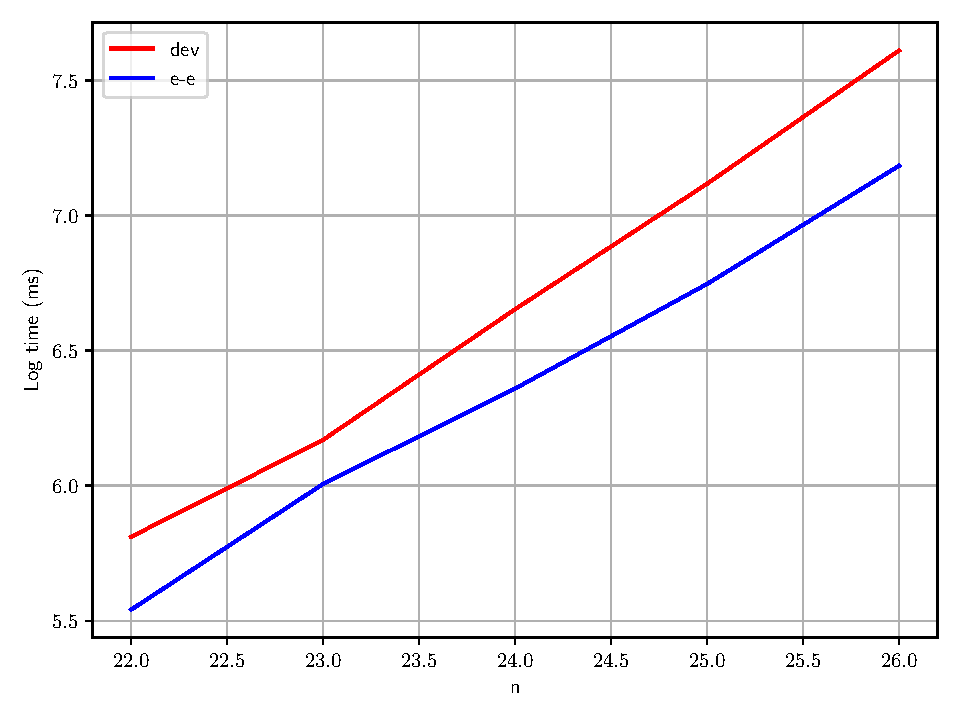
\includegraphics[width=\textwidth]{thesis/img/perf_fib.pdf}
      \caption{Performance}
      \label{fig:perf-fib-graph}
    \end{subfigure}
    \caption{A computationally expensive Hazel program with no holes}
  \end{figure}

  \begin{figure}
    \begin{subfigure}[b]{0.45\textwidth}
      \centering
      \tiny
      \inputhpminted{perf_fib_more_bindings}
      \caption{Source}
      \label{fig:perf-fib-more-bindings}
    \end{subfigure}
    \qquad
    \begin{subfigure}[b]{0.45\textwidth}
      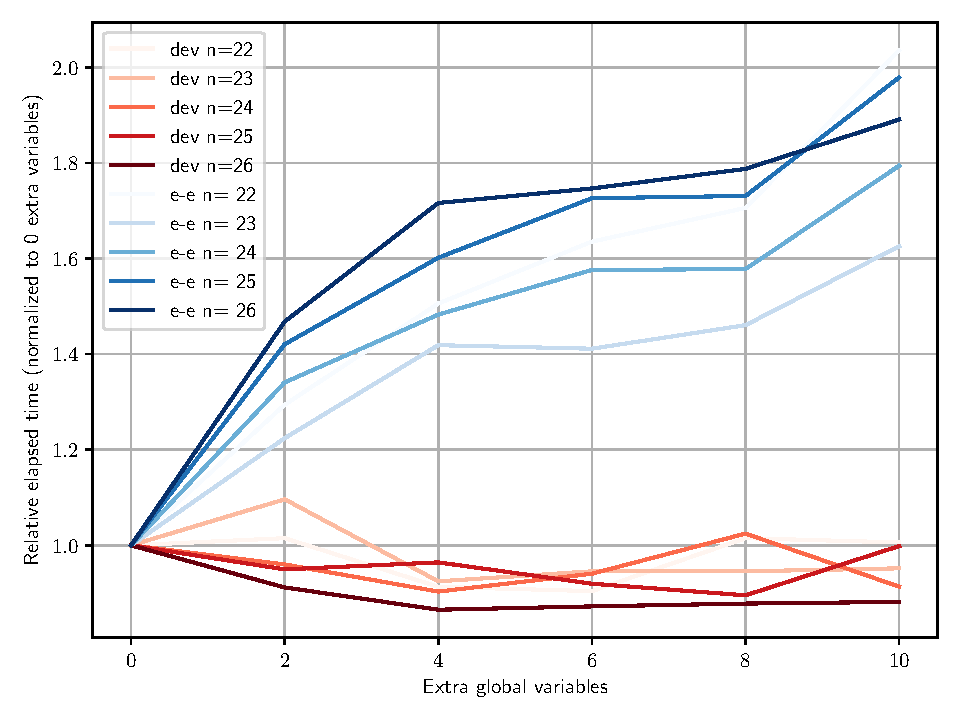
\includegraphics[width=\textwidth]{thesis/img/perf_fib_more_vars.pdf}
      \caption{Performance}
      \label{fig:perf-fib-more-vars-graph}
    \end{subfigure}
    \caption{Adding global bindings to the $\text{fib}(n)$ program}
  \end{figure}

  \begin{figure}
    \begin{subfigure}[b]{0.45\textwidth}
      \centering
      \tiny
      \inputhpminted{perf_fib_more_branches}
      \caption{Source}
      \label{fig:perf-fib-more-branches}
    \end{subfigure}
    \qquad
    \begin{subfigure}[b]{0.45\textwidth}
      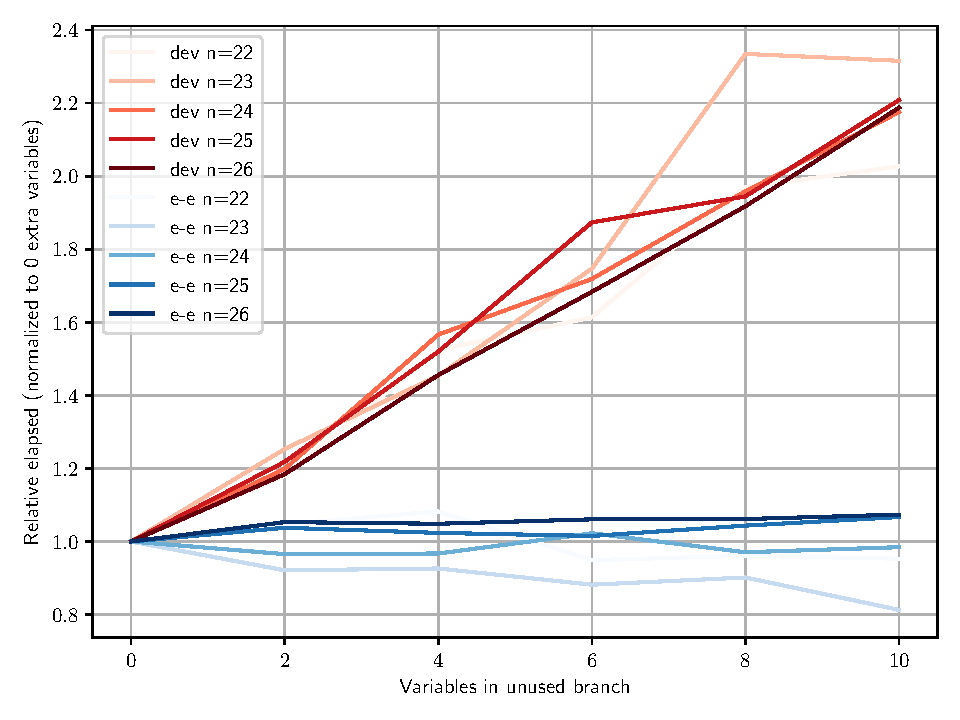
\includegraphics[width=\textwidth]{thesis/img/perf_fib_more_branches.pdf}
      \caption{Performance}
      \label{fig:perf-fib-more-branches-graph}
    \end{subfigure}
    \caption{Adding variable substitutions to unused branches}
  \end{figure}
\end{frame}

\begin{frame}[allowframebreaks]
  \frametitle{Hole numbering motivating example}

  \begin{figure}
    \centering
    \tiny
    \inputhpminted{holes_consecutive}
    \caption{A Hazel program that generates $2^N$ total hole instances}
    \label{fig:hole-renumbering-problem-2}
  \end{figure}

  \begin{figure}
    \centering
    \begin{subfigure}{0.45\textwidth}
      \centering
      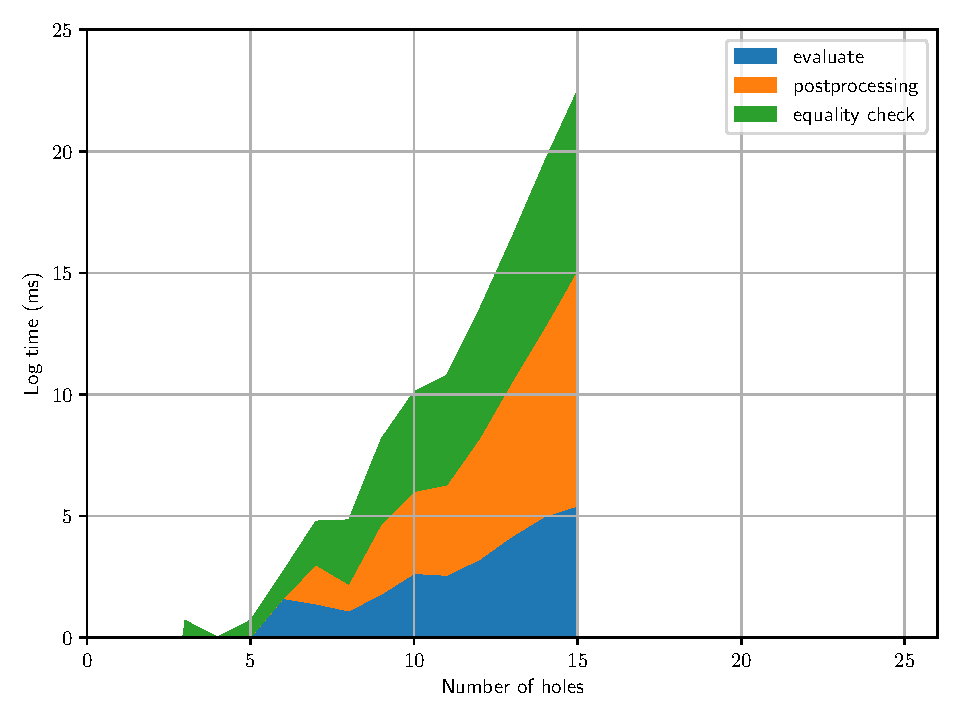
\includegraphics[width=\textwidth]{thesis/img/perf_renum_dev.pdf}
      \caption{\texttt{dev} branch}
      \label{fig:perf-renum-dev}
    \end{subfigure}
    \qquad
    \begin{subfigure}{0.45\textwidth}
      \centering
      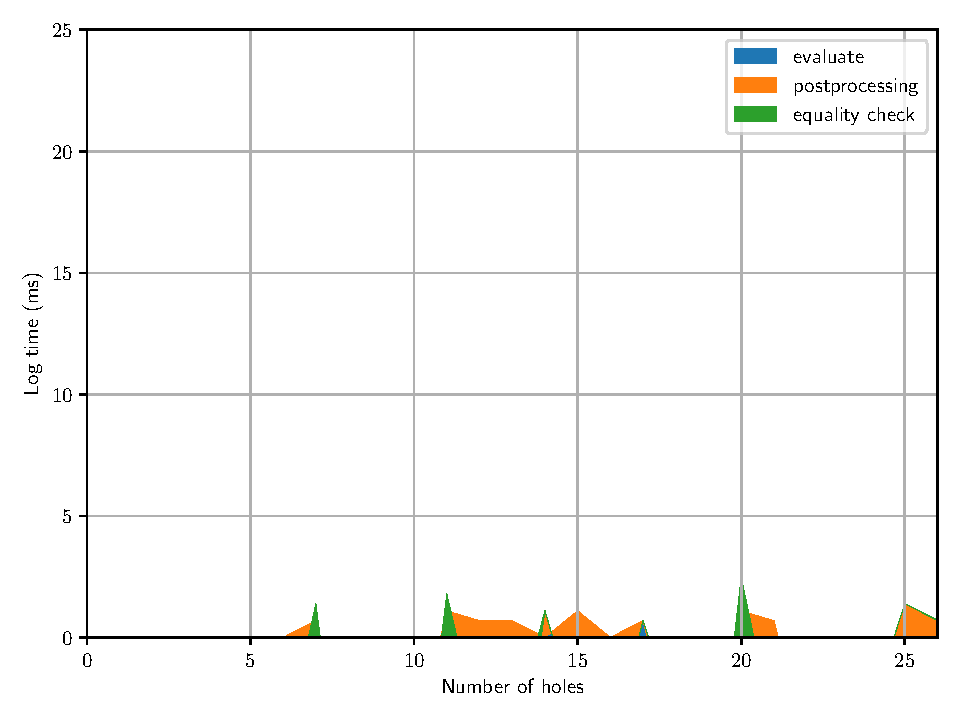
\includegraphics[width=\textwidth]{thesis/img/perf_renum_eev.pdf}
      \caption{\texttt{eval-environment} branch}
      \label{fig:perf-renum-eev}
    \end{subfigure}
    \caption{Performance of evaluating program in \Cref{fig:hole-renumbering-problem}}
    \label{fig:perf-renum}
  \end{figure}
\end{frame}

\begin{frame}[allowframebreaks]
  \frametitle{FAR motivating example}

  \begin{table}
    \centering
    \tiny
    \begin{tabular}{p{10em}cccc}
      \hline
      Program & Steps & Steps & Step $\Delta$ & Cumulative \\
              & & (w/ FAR) & & Step $\Delta$ \\
      \hline\hline
      \inputhnfpminted{far_fib_hist_1} & 7 & - & 0 & 0 \\ \hline
      \inputhnfpminted{far_fib_hist_2} & 12 & 21 & 9 & 9 \\ \hline
      \inputhnfpminted{far_fib_hist_3} & 17 & - & 0 & 9 \\ \hline
      \inputhnfpminted{far_fib_hist_4} & 58 & 69 & 11 & 20 \\ \hline
      \hline
    \end{tabular}
    \caption{A program edit history with an expensive computation}
    \label{fig:far-program-history-fib}
  \end{table}

  \begin{table}
    \centering
    \tiny
    \begin{tabular}{p{10em}cccc}
      \hline
      Program & Steps & Steps & Step $\Delta$ & Cumulative \\
              & & (w/ FAR) & & Step $\Delta$ \\
      \hline\hline
      \inputhnfpminted{far_fib_hist_5} & 4762964 & - & 0 & 20 \\ \hline
      \inputhnfpminted{far_fib_hist_6} & 4762966 & 12 & -4762954 & -4762934 \\ \hline
      \inputhnfpminted{far_fib_hist_7} & 4762966 & 21 & -4762954 & -9525879 \\ \hline
      \inputhnfpminted{far_fib_hist_8} & 4792967 & 13 & -4792954 & -14288813 \\ \hline
      \hline
    \end{tabular}
    \caption{A program edit history with an expensive computation, cont'd.}
    \label{fig:far-program-history-fib-2}
  \end{table}

  \begin{figure}
    \centering
    \begin{subfigure}{0.45\textwidth}
      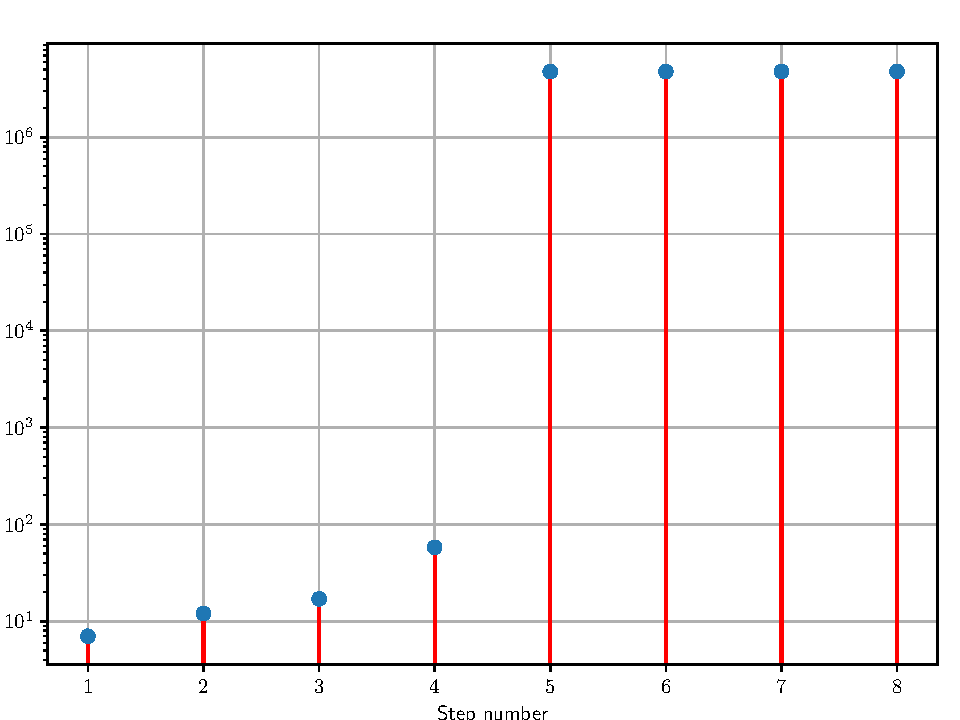
\includegraphics[width=\textwidth]{thesis/img/perf_no_far.pdf}
      \caption{Normal evaluation}
      \label{fig:perf-no-far}
    \end{subfigure}
    \qquad
    \begin{subfigure}{0.45\textwidth}
      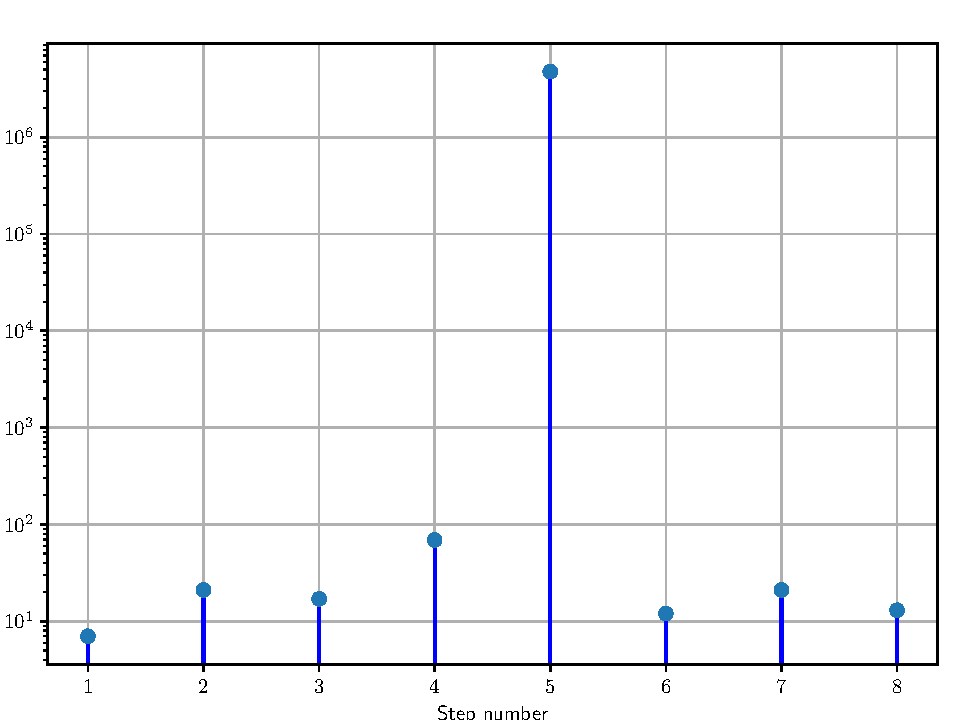
\includegraphics[width=\textwidth]{thesis/img/perf_far.pdf}
      \caption{With one-step FAR}
      \label{fig:perf-far-far}
    \end{subfigure}
    \caption{Number of evaluation steps per edit in \Cref{fig:far-program-history-fib}}
    \label{fig:perf-far}
  \end{figure}
\end{frame}

\section{Discussion and conclusions}

\begin{frame}
  \frametitle{Innovations of this work}

  \begin{description}
  \item[Generalized closures] Useful for evaluation and memoization
  \item[Unique hole closures] Grouping hole instances by environment
  \item[FAR as a generalization of evaluation] Each edit is a $n$-step FAR
  \end{description}
\end{frame}

\begin{frame}
  \frametitle{Metatheory}

  Invariants of the evaluation steps; informally justified

  \begin{description}
  \item[Preservation]
  \item[Evaluation boundary]
  \item[Singular evaluation boundary]
  \item[Substitution postprocessing closures]
  \item[Evaluation with environments correctness]
  \item[Hole numbering postprocessing]
  \item[Fill operation]
  \item[Resume operation]
  \end{description}
\end{frame}

\begin{frame}[allowframebreaks]
  \frametitle{Proposed updates to the evaluation model}

  \begin{figure}
    \centering
    \maxsizebox{\textwidth}{15em}{
      \begin{tikzpicture}
  \node[draw=red] (action) {\mintinline{text}|ModelAction.EditAction.t|};
  \node[draw=black] (syn_action) [below=of action] {\mintinline{text}|Action_Exp.syn_perform|};
  \node[draw=red] (model) [right=80pt of syn_action] {\mintinline{text}|Model.t|};
  \node[draw=black] (elaborate) [below=of syn_action] {\mintinline{text}|Elaborator_Exp.elab|};
  \node[draw=black] (evaluate) [below=of elaborate] {\mintinline{text}|Evaluator.evaluate|};
  \node[draw=black] (renumber) [below=of evaluate] {\mintinline{text}|EvalPostprocess.postprocess|};
  \node[draw=red] (undo_hist) [below=of model] {\mintinline{text}|UndoHistory.t|};
  \node[draw=red] (result) [below= of undo_hist] {\mintinline{text}|Result.t|};

  \draw[->,thick] (action) -- (syn_action) node [midway,left] {$\alpha$};
  \draw[->,thick] (model) -- (syn_action) node [midway,above] {\mintinline{text}|Program.t|};
  \draw[->,thick] (syn_action) -- (elaborate) node [midway,left] {$e$};
  \draw[->,thick] (elaborate) -- (evaluate) node [midway,left] {$d_{uneval}$};
  \draw[->,thick] (evaluate) -- (renumber) node [midway,left] {$d_{eval}$};
  \draw[->,thick] (evaluate) -- (result) node [midway,above] {$d_{eval}$};
  \draw[->,thick] (renumber) -- (result) node [midway,below right] {$d_{renumbered},\hci$};
  \draw[->,thick] (result) -- (undo_hist);
  \draw[->,thick] (undo_hist) -- (model);
\end{tikzpicture}

    }
    \caption{Previous evaluation model}
    \label{fig:prev-evaluation-call-graph}
  \end{figure}

  \begin{figure}
    \centering
    \maxsizebox{\textwidth}{15em}{
      \begin{tikzpicture}
  \node[draw=red] (action) {\mintinline{text}|ModelAction.EditAction.t|};
  \node[draw=black] (syn_action) [below=of action] {\mintinline{text}|Action_Exp.syn_perform|};
  \node[draw=red] (model) [right=60pt of syn_action] {\mintinline{text}|Model.t|};
  \node[draw=black] (elaborate) [below=of syn_action] {\mintinline{text}|Elaborator_Exp.elab|};
  \node[draw=blue] (detect_fill) [below=of elaborate] {\mintinline{text}|DHExpDiff.diff_dhexp|};
  \node[draw=blue] (preprocess) [below left=of detect_fill] {\mintinline{text}|FillAndResume.preprocess|};
  \node[draw=black] (evaluate) [below=60pt of detect_fill] {\mintinline{text}|Evaluator.evaluate|};
  \node[draw=black] (renumber) [below=of evaluate] {\mintinline{text}|EvalPostprocess.postprocess|};
  \node[draw=red] (undo_hist) [below=of model] {\mintinline{text}|UndoHistory.t|};
  \node[draw=red] (result) [below= of undo_hist] {\mintinline{text}|Result.t|};

  \draw[->,thick] (action) to[] node [midway,left] {$\alpha$} (syn_action);
  \draw[->,thick] (model) to[bend right=5] node [midway,above,xshift=10pt] {\mintinline{text}|Program.t|} (syn_action);
  \draw[->,thick] (syn_action) to[] node [midway,left] {$e$} (elaborate);
  \draw[->,thick] (elaborate) to[] node [midway,left] {$d_{uneval}$} (detect_fill);
  \draw[->,thick] (detect_fill) to[] node [midway,right] {no fill diff} (evaluate);
  \draw[->,thick,blue] (detect_fill) to[bend right=10] node [midway,above left] {$u,d$} (preprocess);
  \draw[->,thick,blue] (preprocess) to[bend right=10] node [midway,below left] {$d_{preprocess}$} (evaluate);
  \draw[->,thick] (evaluate) to[] node [midway,left] {$d_{eval}$} (renumber);
  \draw[->,thick] (evaluate) to[bend right=15] node [midway,above left] {$d_{eval}$} (result);
  \draw[->,thick] (renumber) to[bend right=10] node [midway,below right] {$d_{postprocess},\hci$} (result);
  \draw[->,thick,blue] (undo_hist) to[bend left=20] node [xshift=10pt,above left] {\mintinline{text}|list(Program.t)|} (detect_fill);
  \draw[->,thick] (result) to[] (undo_hist);
  \draw[->,thick] (undo_hist) to[] (model);
\end{tikzpicture}

%%% Local Variables:
%%% mode: latex
%%% TeX-master: "main"
%%% End:

    }
    \caption{Proposed evaluation model}
    \label{fig:current-evaluation-call-graph}
  \end{figure}
\end{frame}

\begin{frame}
  \frametitle{Future work}

  \begin{description}
  \item[Fully automatic FAR] Integrate FAR into the Hazel MVC model
  \item[$n$-step FAR] Integrate edit history into FAR
  \item[Formal evaluation of metatheory] Check coverage and correctness of metatheorems using Agda
  \item[User editing studies] Gather data on ``true'' performance impact
  \end{description}
\end{frame}

\begin{frame}
  \frametitle{Conclusions}

  \begin{description}
  \item[Evaluation with environments] Expected performance gains, implementation remains functionally pure
  \item[Generalized closures] Simplify many parts of the implementation, also useful for FAR
  \item[Memoization of environments] Applicable for postprocessing, equality checking, resume operation
  \item[FAR PoC] Including $n$-step detection, re-evaluation of closures
  \item[Plausible metatheory] For future work in Agda
  \end{description}
\end{frame}

\begin{frame}[allowframebreaks]
  \frametitle{References}

  \tiny
  \bibliographystyle{unsrt}
  \bibliography{thesis/refs}
\end{frame}

\end{document}

%%% Local Variables:
%%% mode: latex
%%% TeX-master: t
%%% End:
